%\begin{wrapfigure}[0]{r}[-4cm]{3cm}
% \vspace{-6cm}
% 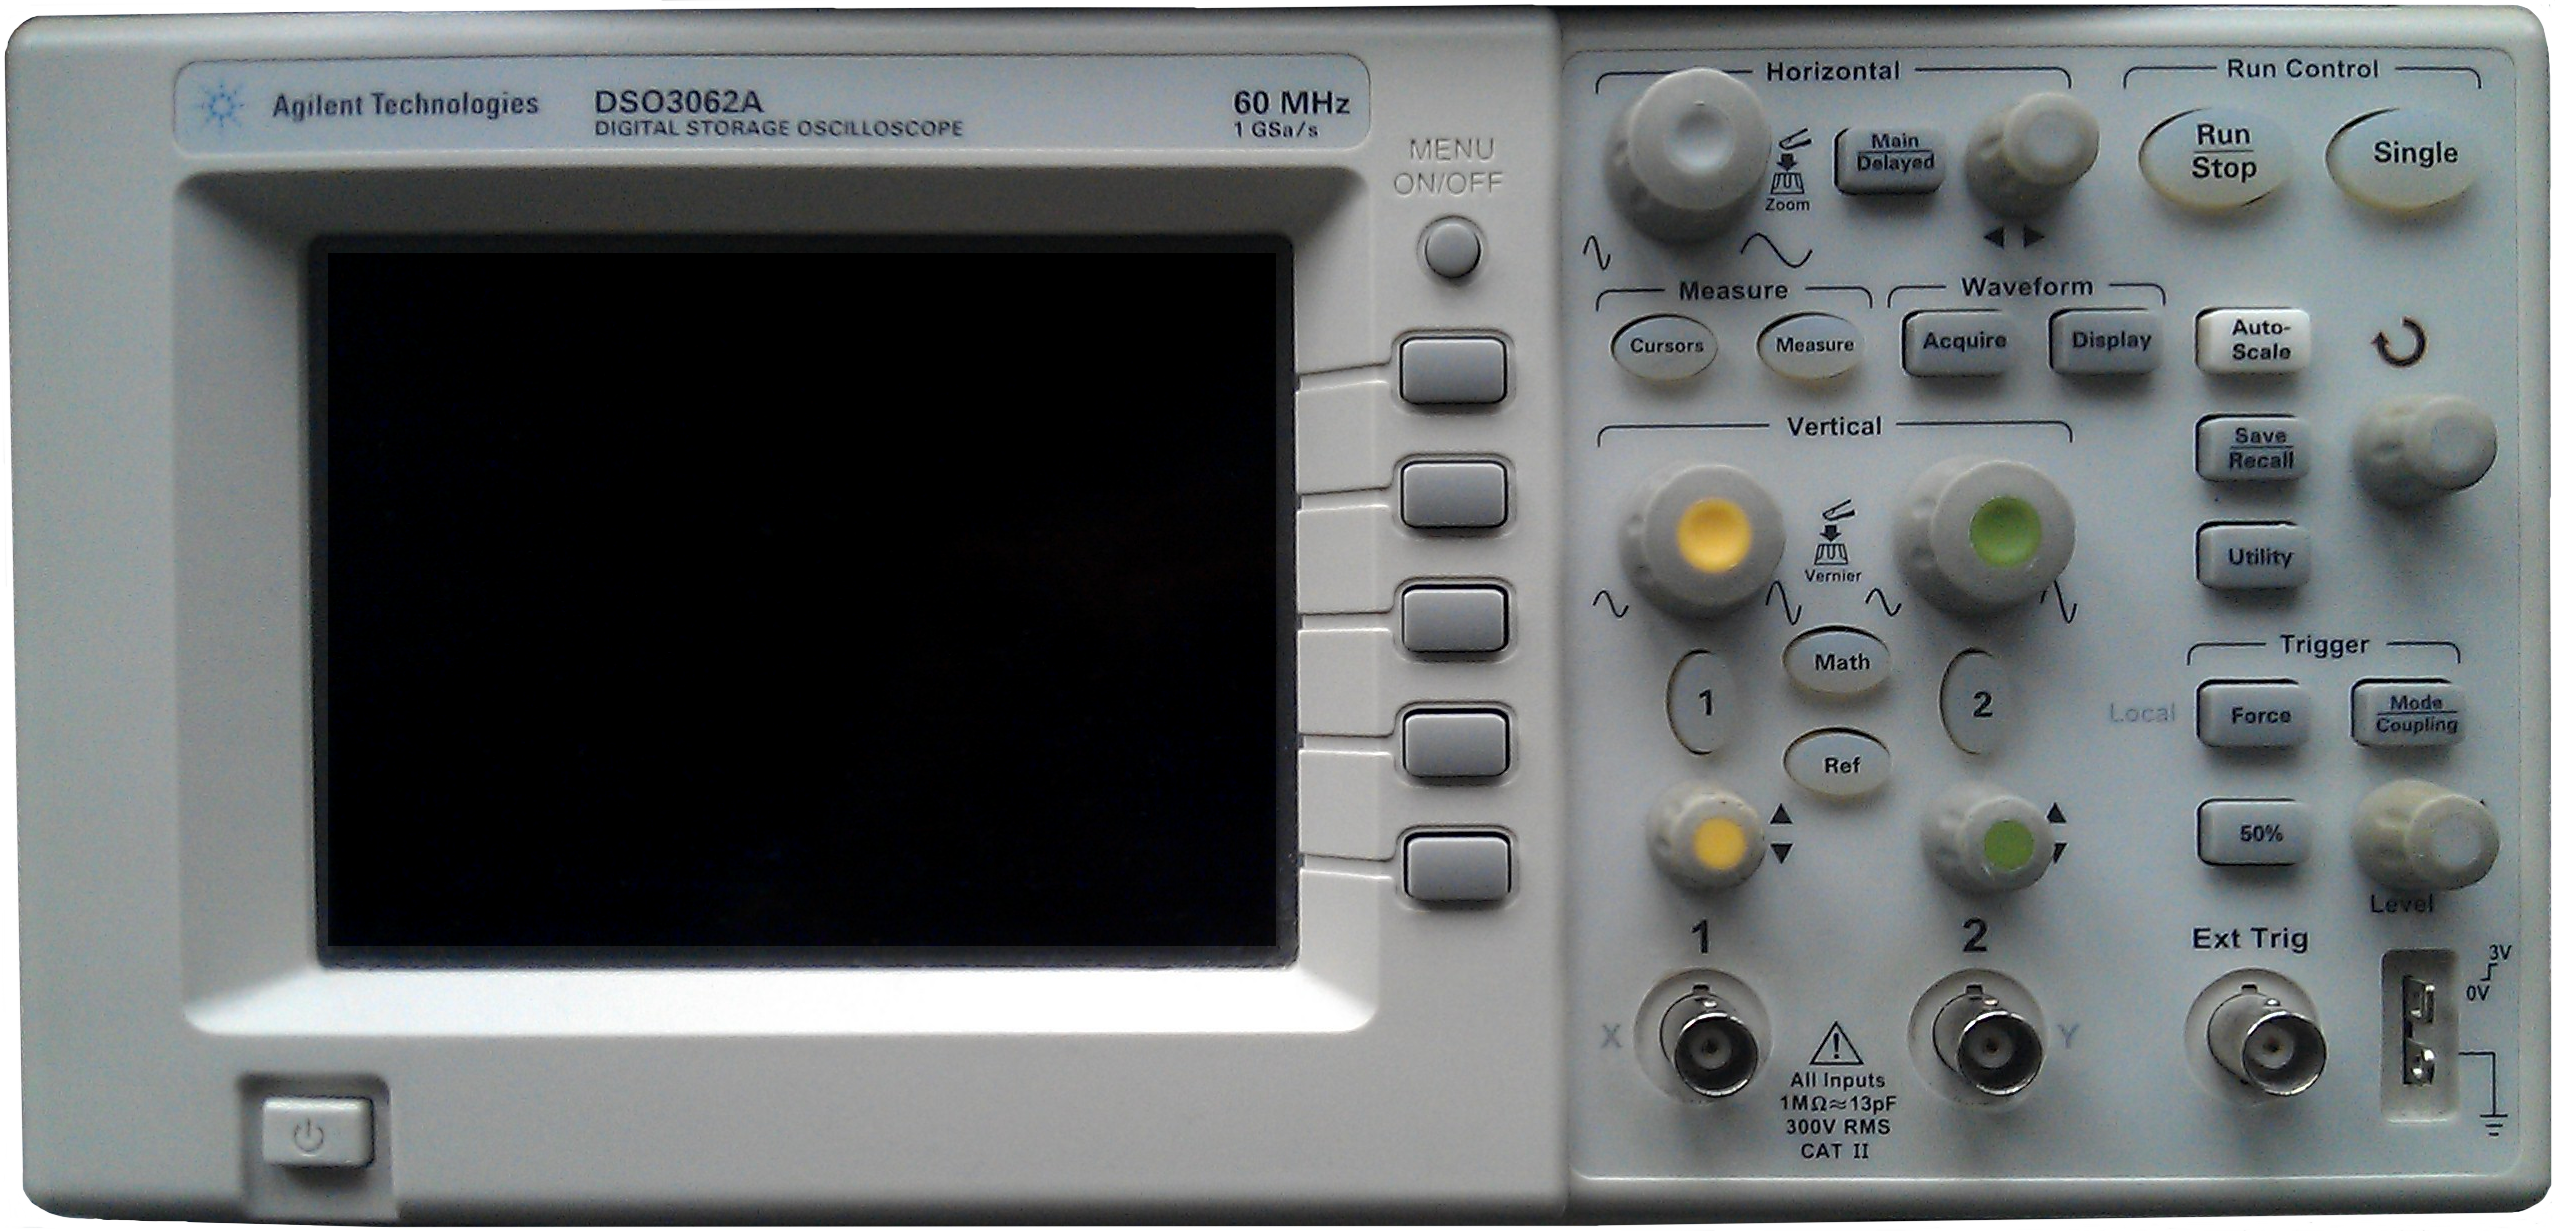
\includegraphics[scale=0.08]{Messtechnik/Bilder/oszi_foto.png}
% \vspace{-6cm}
%\end{wrapfigure}

\section*{Theorie- und Prüfungsfragen} 

\mucho{1}{TD612}
{Wie verhält sich die Frequenz eines Oszillators bei Temperaturanstieg, wenn die Kapazität des Schwingkreiskondensators mit dem Temperaturanstieg ebenfalls ansteigt?}%Frage
{Die Frequenz bleibt stabil.}%A
{Die Schwingungen reißen ab (Aussetzer).}%B
{Die Frequenz erhöht sich.}%C
{Die Frequenz verringert sich.}%D
{D}%Lösung

\mucho{2}{TD420}
{Welche Merkmale hat ein HF-Leistungsverstärker im A-Betrieb?}%Frage
{Wirkungsgrad $80$ bis $87 \%$, hoher Oberwellenanteil, der Ruhestrom ist fast null.}%A
{Wirkungsgrad bis zu $70 \%$, geringer Oberwellenanteil, geringer bis mittlerer Ruhestrom.}%B
{Wirkungsgrad bis zu $80 \%$, geringer Oberwellenanteil, sehr geringer Ruhestrom.}%C
{Wirkungsgrad ca. $40 \%$, geringst möglicher Oberwellenanteil, hoher Ruhestrom.}%D
{D}%Lösung

\mucho{3}{TD421}
{Welche Merkmale hat ein HF-Leistungsverstärker im B-Betrieb?}%Frage
{Wirkungsgrad ca. $40 \%$, geringst möglicher Oberwellenanteil, hoher Ruhestrom.}%A
{Wirkungsgrad bis zu $70 \%$, geringer Oberwellenanteil, geringer bis mittlerer Ruhestrom.}%B
{Wirkungsgrad bis zu $80 \%$, geringer Oberwellenanteil, sehr geringer Ruhestrom.
}%C
{Wirkungsgrad $80$ bis $87 \%$, hoher Oberwellenanteil, der Ruhestrom ist fast null.
}%D
{C}%Lösung


\mucho{4}{TD422}
{ Welche Merkmale hat ein HF-Leistungsverstärker im C-Betrieb?}%Frage
{Wirkungsgrad bis zu $70 \%$, geringer Oberwellenanteil, geringer bis mittlerer Ruhestrom.}%A
{Wirkungsgrad $80$ bis $87 \%$, hoher Oberwellenanteil, der Ruhestrom ist fast null.}%B
{Wirkungsgrad bis zu $80 \%$, geringer Oberwellenanteil, sehr geringer Ruhestrom.}%C
{Wirkungsgrad ca. $40 \%$, geringst möglicher Oberwellenanteil, hoher Ruhestrom.}%D
{B}%Lösung


\mucho{5}{TB904}
{Die äquivalente (effektive) Strahlungsleistung (ERP) ist}%Frage
{das Produkt aus der Leistung, die unmittelbar der Antenne zugeführt wird und ihrem Gewinnfaktor in einer Richtung, bezogen auf den Halbwellendipol.}%A
{das Produkt aus der Leistung, die unmittelbar der Antenne zugeführt wird und ihrem Gewinnfaktor in einer Richtung, bezogen auf den isotropen Kugelstrahler.}%B
{die durchschnittliche Leistung, die ein Sender unter normalen Betriebsbedingungen während einer Periode der Hochfrequenzschwingung bei der höchsten Spitze der Modulationshüllkurve der Antennenspeiseleitung zuführt.}%C
{die durchschnittliche Leistung, die ein Sender unter normalen Betriebsbedingungen an die Antennenspeiseleitung während eines Zeitintervalls abgibt, das im Verhältnis zur Periode der tiefsten Modulationsfrequenz ausreichend lang ist.}%D
{A}%Lösung

\mucho{6}{TB905}
{Die äquivalente isotrope Strahlungsleistung (EIRP) ist}%Frage
{das Produkt aus der Leistung, die unmittelbar der Antenne zugeführt wird und ihrem Gewinnfaktor in einer Richtung, bezogen auf den isotropen Kugelstrahler.}%A
{das Produkt aus der Leistung, die unmittelbar der Antenne zugeführt wird und ihrem Gewinnfaktor in einer Richtung, bezogen auf den Halbwellendipol.}%B
{die durchschnittliche Leistung, die ein Sender unter normalen Betriebsbedingungen während einer Periode der Hochfrequenzschwingung bei der höchsten Spitze der Modulationshüllkurve der Antennenspeiseleitung zuführt.}%C
{die durchschnittliche Leistung, die ein Sender unter normalen Betriebsbedingungen an die Antennenspeiseleitung während eines Zeitintervalls abgibt, das im Verhältnis zur Periode der tiefsten Modulationsfrequenz ausreichend lang ist.}%D
{A}%Lösung



\mucho{7}{TD603}
{Bei dieser Schaltung handelt es sich um\\
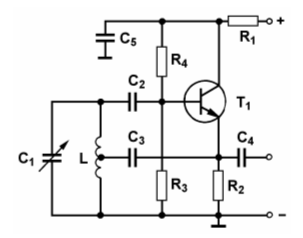
\includegraphics[scale=0.5]{Oszillator/Bilder/TD603.png}}%Frage
{einen LC-Oszillator in induktiver Dreipunktschaltung.}%A
{einen LC-Oszillator in kapazitiver Dreipunktschaltung.}%B
{einen Oberton-Oszillator in Kollektorschaltung.}%C
{einen Oberton-Oszillator in Emitterschaltung.}%D
{A}%Lösung


\mucho{8}{TD605}
{Bei dieser Oszillatorschaltung handelt es sich um einen kapazitiv rückgekoppelten Quarz-Oszillator in\\
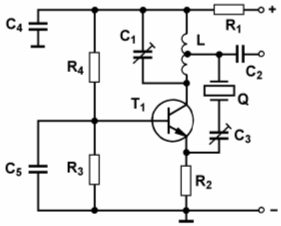
\includegraphics[scale=0.5]{Oszillator/Bilder/TD605.png}}%Frage
{Basisschaltung, in der der Quarz in Serienresonanz betrieben wird.}%A
{Basisschaltung, in der der Quarz in Parallelresonanz betrieben wird.}%B
{Emitterschaltung, in der der Quarz in Parallelresonanz betrieben wird.}%C
{Emitterschaltung, in der der Quarz in Serienresonanz betrieben wird.}%D
{A}%Lösung